\chapter{Ristrutturazione dello schema concettuale}

    \section{Analisi delle Ridondanze}

    In questa fase abbiamo rilevato che l'entità "Collana", potesse essere gestita da una "View" in quanto la "Collana" in se può essere rappresentata da una interrogazione sulla base di dati che rappresenta una collezione di "Libri" con caratteristiche comuni.
    Inoltre dato l'utilizzo frequente dell'informazione della quantità di libri in una serie, si è optato per l'introduzione dell'attributo "NumLibri" sull'entità "Serie", anche essendo esso ridondante, in quanto derivabile da una interrogazione.
    
    \section{Eliminazione delle Generalizzazioni}

    Le generalizzazioni riscontrate nello schema concettuale sono: "Pubblicazione", "Libro", "Presentazione", "Piattaforma" e "Acquisto". Ognuna di esse dovrà essere opportunamente ristrutturata.\\
    
    \begin{itemize}
        \item La generalizzazione "Pubblicazione" verrà risolta accorpando il padre nelle figlie, in quanto è necessaria una marcata distinzione per le entità "Libro" e "Articolo scientifico" che saranno caratterizzate dai loro  attributi propri e acquisiranno gli attributi di "Pubblicazione". Per l'associazione "Disponibile\_P", la quale definita tra "Pubblicazione" e "Acquisto", verrà rimpiazzata con "Disponibile\_L" tra "Libro" e "Acquisto" e "Disponibile\_A" tra "Articolo scientifico" e "Acquisto".
        \item La generalizzazione "Libro" verrà risolta accorpando le entità figlie nel padre, in quanto non ci interessa trattare separatamente le entità figlie "Didattico" e "Romanzo". L'entità "Libro" acquisirà gli attributi delle sue entità figlie con l'aggiunta dell'attributo tipo per differenziare le due possibili istanze di "Libro". 
        \item La generalizzazione "Presentazione" verrà risolta accorpando le figlie nel padre, in quanto non sarà necessaria una distinzione per le entità figlie "Libreria" e "Sala", dunque  i loro attributi saranno acquisiti da "Presentazione" con l'aggiunta dell'attributo tipo per differenziare le due possibili istanze di "Presentazione". L'associazione tra "Presentazione" e "Libro" rimarrà invariata.
        \item  La generalizzazione "Piattaforma" verrà risolta accorpando le figlie nel padre, in quanto non sarà necessaria una distinzione per le entità "Conferenza" e "Rivista", dunque  i loro attributi saranno acquisiti da "Piattaforma" con l'aggiunta dell'attributo tipo per differenziare le due possibili istanze di "Piattaforma". L'associazione tra "Piattaforma" e "Articolo scientifico" rimarrà invariata.
        \item  La generalizzazione "Acquisto" verrà risolta accorpando le figlie nel padre, in quanto non sarà necessaria una distinzione per le entità "Online" e "Libreria", dunque  i loro attributi saranno acquisiti da "Acquisto" con l'aggiunta dell'attributo tipo per differenziare le due possibili istanze di "Acquisto". L'associazione tra "Acquisto" e "Libro" rimarrà invariata.
    \end{itemize}


    

    \section{Eliminazione degli attributi multi valore}

    Gli attributi multi valore presenti nello schema concettuale sono: "Autore" e "Fruizione" entrambi presenti nell'entità "Libro".     
    \begin{itemize}
        \item L'attributo multiplo "Autore" può rappresentare nel diagramma ER uno o più autori, dunque abbiamo deciso di trasformarlo in un attributo semplice di tipo stringa in cui tutti gli autori  vengono rappresentati separati da una virgola. Questa scelta è stata adoperata in quanto non ci interesserà tenere traccia ed utilizzare gli autori singolarmente, inoltre i libri spesso vengono scritti da un singolo autore, ma nell'eventualità di altri autori, essi saranno rappresentati dopo l'autore e saranno intesi come co-autori.
        \item L'attributo multiplo "Fruizione"  assume le modalità di consumazione di un libro (es cartaceo, digitale e audiolibro). Esso verrà trasformato in una stringa contenente le modalità disponibili per il libro separate da una virgola, in modo da non vincolarci sulle sue modalità ma avere la possibilità di inserire in futuro una nuova modalità non presente in questo momento.
    \end{itemize}
    \section{Eliminazione degli attributi strutturati}
     L'attributo strutturato presente nello schema concettuale è l' attributo "Indirizzo". Esso è presente nell'entità "Conferenza", nell'entità "Acquisto" e nell'entità "Presentazione".   

     \begin{itemize}
         \item L'attributo "Indirizzo" è composto dagli attributi "Via","Città" e "Cap". Sarà trasformato in un'unica stringa in quanto nella gestione della nostra realtà d'interesse non è importante tenere traccia separatamente di ogni attributo ma unicamente del singolo indirizzo.
     \end{itemize}
    \section{Vincoli}
    I vincoli individuati della nostra realtà di interesse sono :\\
    \begin{itemize}
        \item Vincoli di integrità impliciti
            \begin{itemize}
                \item Vincoli di chiave primaria: Spiegati in \hyperref[sec:PK]{\textit{"Identificazione delle chiavi primarie}"}
                \item Vincoli di chiave esterna: Spiegati in \hyperref[sec:Mapping]{\textit{"Mapping"}}
            \end{itemize}
        \item Vincoli di integrità espliciti
            \begin{itemize}
                {\bf\item Controllo\_Date\_Conferenza (Conferenza):}\\(DataI $<=$ DataF)
                \\\textit{Vincolo che impedisce ad una conferenza di avere una data di inizio precedente alla sua data di fine.}
                
                 \item  {\bf Numero\_Pagine\_ArticoloS (Articolo Scientifico) }:\\ (NumPagine $>$ 0 and \\(Fruizione LIKE '\%Cartaceo\%' or Fruizione LIKE '\%Digitale\%'))or\\(NumPagine = 0 and (Fruizione LIKE 'AudioLibro')))
                 \\\textit{Vincolo che impedisce ad un Articolo Scientifico di avere un numero di pagine negativo e una fruizione "Cartacea" e/o "Digitale" oppure un numero di pagine diverso da zero e la sua unica fruizione non è "Audiolibro".}
                 
                 {\bf\item Fruizione (Acquisto):} \\ ((url IS NULL) != (indirizzo IS NULL)) and\\ ((Tipo = 'Sito web') and (url is not null) or\\ (Tipo = 'Libreria') and (Indirizzo is not null))
                 \\\textit{Vincolo che deriva dalla generalizzazione, il valore del tipo deve essere  "Libreria" o "Online" e di conseguenza avere un "indirizzo" per la "Libreria" e un "url" per "Online" ed il contrario non valorizzabile.}

                \item {\bf Controllo\_Completata (Serie)}: \\((Completata = TRUE and NumLibri $>$ 1) or Completata = FALSE),
                 \\\textit{Vincolo che impone ad una serie completa di avere almeno due libri altrimenti dovrà essere non completa.}

                \item {\bf Controllo\_NumLibri (Serie)}; \\NumLibri $>=$ 0
                 \\\textit{Vincolo che impone ad una serie di avere un numero non negativo di libri}
                
                \item {\bf Tipo\_Libro (Libro)}:\\ ((tipo = 'Didattico') and  (Materia is not null)) or \\((tipo = 'Romanzo') and (materia is null))),
                 \\\textit{Vincolo che deriva dalla generalizzazione, il  valore del tipo deve essere "Didattico" o "Romanzo", se il libro è "didattico" deve possedere una materie, altrimenti un libro "romanzo" non deve possedere una materia. }

                \item  {\bf Numero\_Pagine\_Libro (Libro)}:\\ (NumPagine $>$ 0 and \\(Fruizione LIKE '\%Cartaceo\%' or Fruizione LIKE '\%Digitale\%'))or\\(NumPagine = 0 and (Fruizione LIKE 'AudioLibro')))
                 \\\textit{Vincolo che impedisce ad un Libro di avere un numero di pagine negativo e una fruizione "Cartacea" e/o "Digitale" oppure un numero di pagine diverso da zero e la sua unica fruizione non è "Audiolibro".}

            \end{itemize}
    \end{itemize}
  
     

        
       
  
    

    \newpage
    \section{Identificazione delle chiavi primarie}
   \begin{center}
   \label{sec:PK}

    \begin{tabular}{ | m{5cm} | m{5cm}| m{6cm} | } 
        \hline
             {\bf Entità} & {\bf Chiave Primaria}  & {\bf Descrizione pk}\\ 
         \hline 

              Libro &  ISBN  & Codice di 13 cifre che identifica univocamente un "Libro".\\ 
        \hline
              Articolo Scientifico & DOI & Codice di caratteri che identifica univocamente un "Articolo scientifico".\\ 
        \hline
            Conferenza &  CodC  & Codice di cifre che identifica univocamente una "Conferenza", aggiunto data la mancanza in "Conferenza" di un attributo univoco.\\ 
       \hline
      
           Rivista & Nome , Data & Nome e data di uscita della "Rivista" che insieme identificano univocamente una "Rivista".\\ 
        \hline
            \end{tabular}
       \begin{tabular}{ | m{5cm} | m{5cm}| m{6cm} | } 
       \hline
           Presentazione  & CodP & Codice di cifre che identifica univocamente una "Presentazione", aggiunto data la mancanza in "Presentazione" di un attributo univoco.\\ 
        \hline
           Serie & CodS & Codice di cifre che identifica univocamente una "Serie", aggiunto data la mancanza in "Serie" di un attributo univoco.\\ 
     
       \hline
           Acquisto & CodA & Codice di cifre che identifica univocamente un' "Acquisto", aggiunto data la mancanza in "Acquisto" di un attributo univoco.\\ 
        \hline
           Utente & Email & Email dell'"Utente" unica, lo identifica univocamente.\\ 
        \hline
       
     \end{tabular}
 \end{center}
 
    \newpage
    \section{Schema ristrutturato ER}

      \begin{flushleft}
            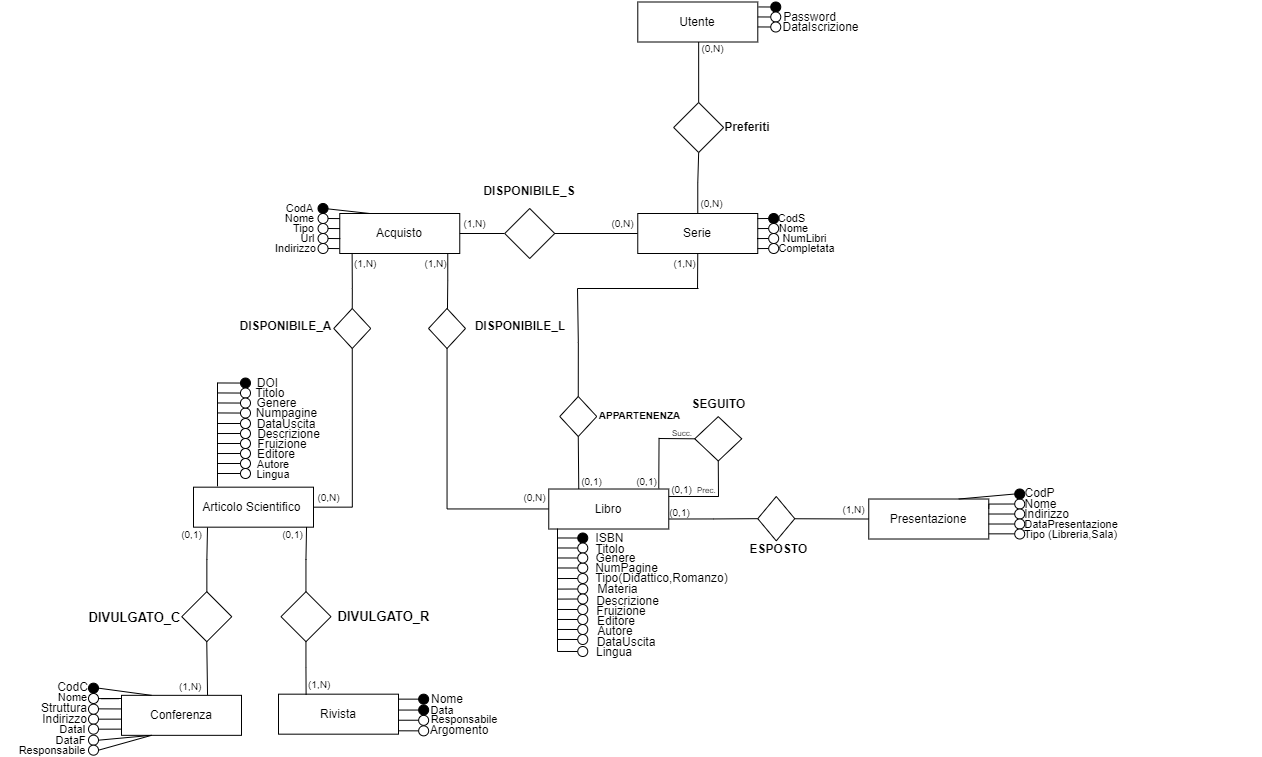
\includegraphics[width=0.98\textwidth]{Immagini/DiagrammaErRistrutturato.png}
        \end{flushleft}
    
    \newpage

    \section{Schema ristrutturato UML}

          \begin{flushleft}
            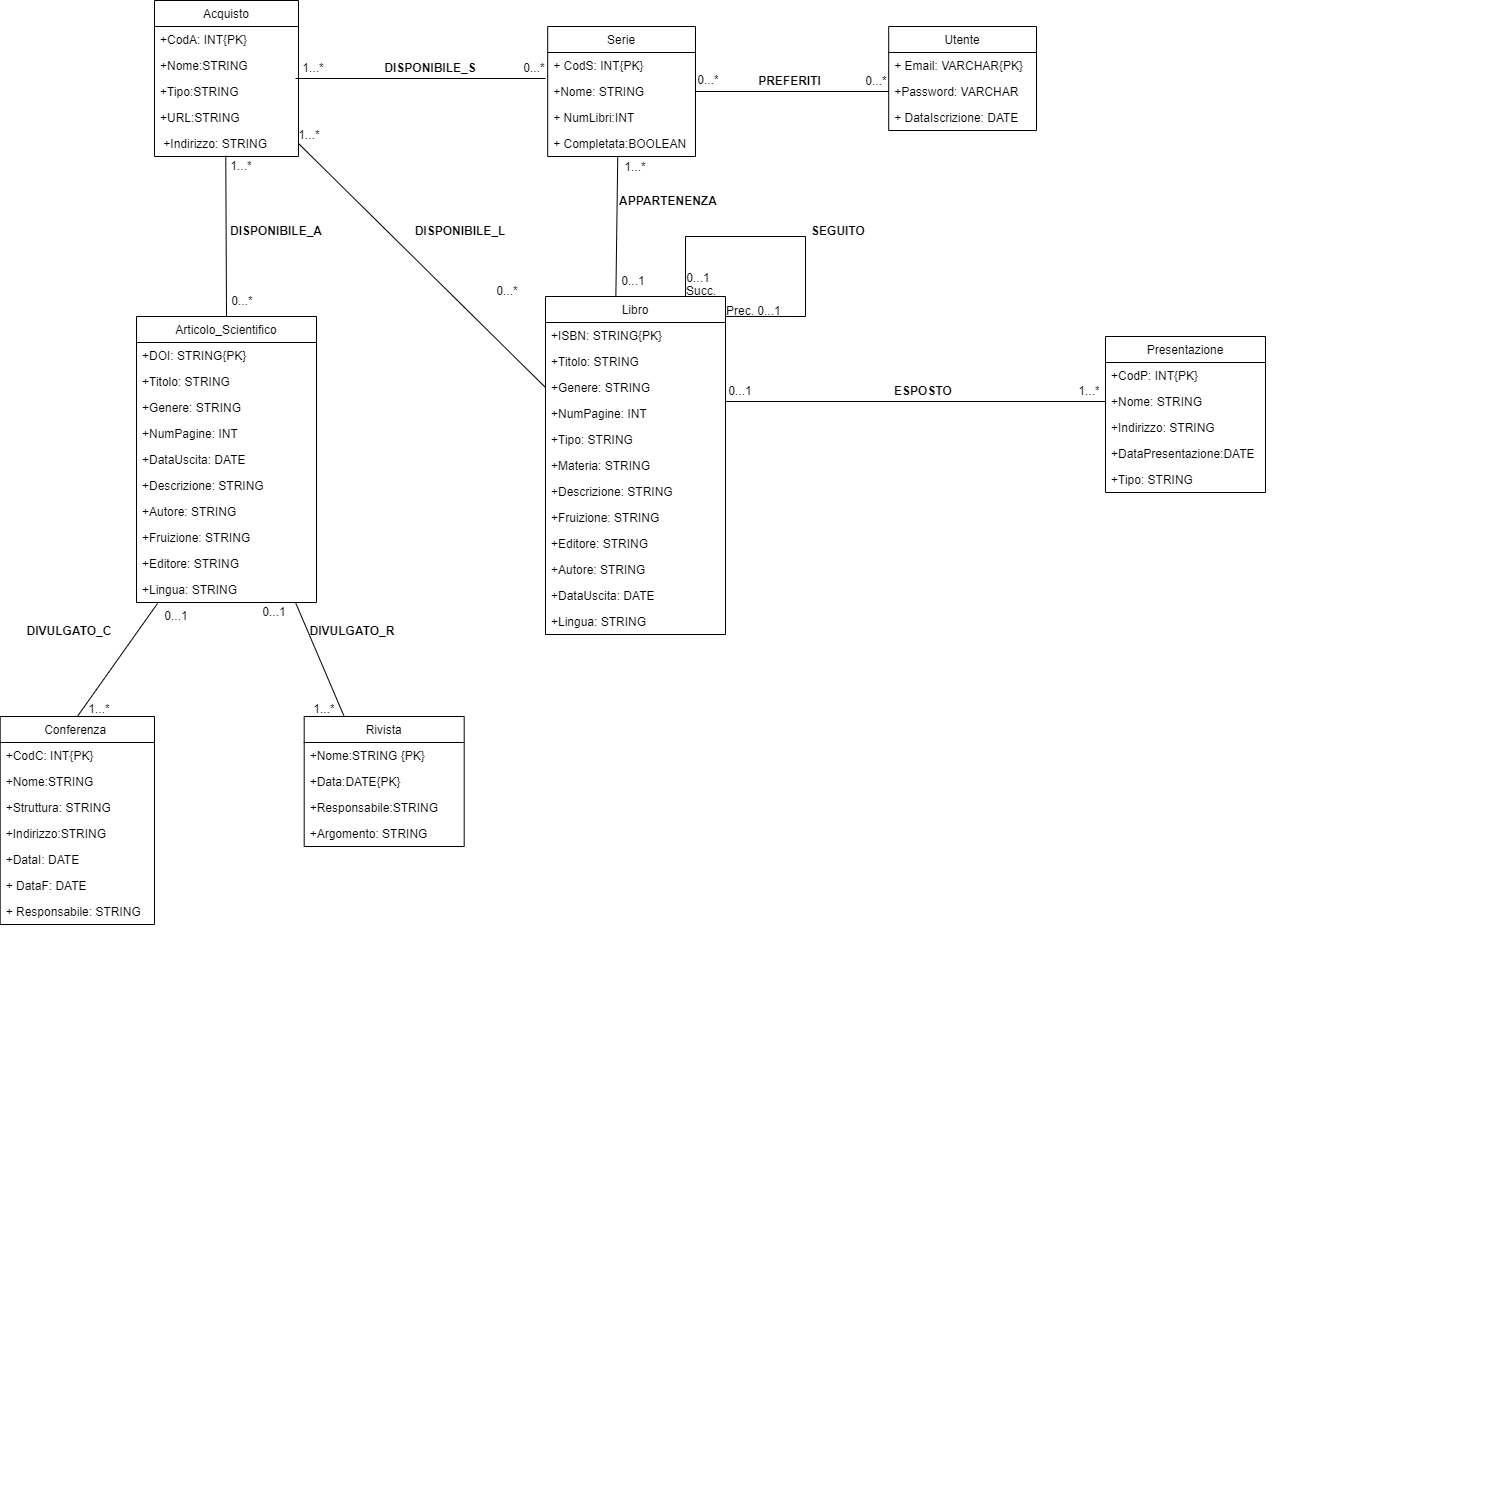
\includegraphics[width=0.98\textwidth]{Immagini/DiagrammaUMLRistrutturato.png}
        \end{flushleft}

    